\subsection{GCC}

\RU{Теперь скомпилируем то же самое компилятором GCC 4.4.1 в Linux}
\EN{Now let's try to compile the same \CCpp code in the GCC 4.4.1 compiler in Linux}: \TT{gcc 1.c -o 1}

\RU{Затем, при помощи \IDA{}, посмотрим, как создалась функция \main.}
\EN{Next, with the assistance of the \IDA disassembler, let's see how the \main function was created.} 

(\IDA, \RU{как и MSVC, показывает код в Intel-синтаксисе}\EN{like MSVC, uses Intel-syntax}).
% Since only GCC listing is included bellow an IDA screenshot or listing could be benfitial to illustrate the above statements
% I have included an image and sample latex segment bellow for review
%
%\begin{figure}[H]
%\centering
%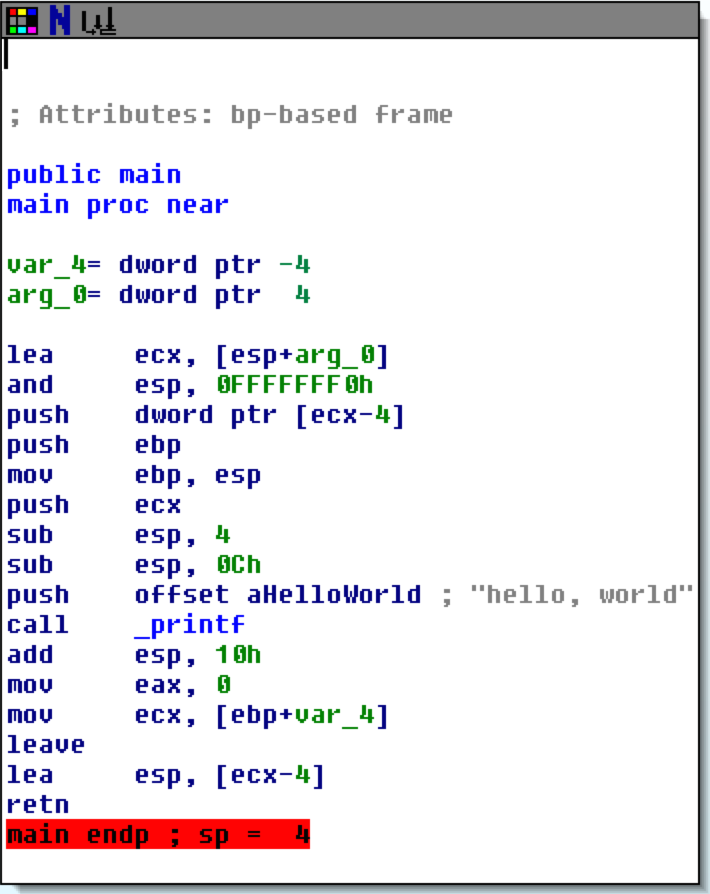
\includegraphics[scale=\FigScale]{patterns/01_helloworld/IDA-helloworld-32.png}
%\caption{\IDA: \TT{hello world}}
%\label{fig:IDA_helloworld_32}
%\end{figure}

N.B. \RU{Мы также можем заставить GCC генерировать листинги в этом формате при помощи ключей}
\EN{We could also have GCC produce assembly listings in Intel-syntax by applying the options} 
\TT{-S -masm=intel}

\begin{lstlisting}[caption=GCC]
main            proc near

var_10          = dword ptr -10h

                push    ebp
                mov     ebp, esp
                and     esp, 0FFFFFFF0h
                sub     esp, 10h
                mov     eax, offset aHelloWorld ; "hello, world\n"
                mov     [esp+10h+var_10], eax
                call    _printf
                mov     eax, 0
                leave
                retn
main            endp
\end{lstlisting}

\index{Function prologue}
\index{x86!\Instructions!AND}
\RU{Почти то же самое. 
Адрес строки ``hello, world'', лежащей в сегменте данных, вначале сохраняется в \EAX, затем записывается в стек.
А еще в прологе функции мы видим \TT{AND ESP, 0FFFFFFF0h} ~--- 
эта инструкция выравнивает значение в \ESP по 16-байтной границе, делая все значения 
в стеке также выровненными по этой границе (процессор более эффективно работает с переменными, расположенными
в памяти по адресам кратным 4 или 16)\footnote{\URLWPDA}.}
\EN{The result is almost the same.
The address of the ``hello, world'' string (stored in the data segment) is loaded in the \EAX register first and then it is saved onto the stack.
In addition, the function prologue contains \TT{AND ESP, 0FFFFFFF0h}~---this 
instruction aligns the \ESP register value on a 16-byte boundary.
This results in all values in the stack being aligned the same way (The CPU performs better if the values it is dealing with are located in memory at addresses aligned 
on a 4- or 16-byte boundary)\footnote{\URLWPDA}.}

\index{x86!\Instructions!SUB}
\TT{SUB ESP, 10h} \RU{выделяет в стеке 16 байт. Хотя, как будет видно далее, здесь достаточно только 4.}
\EN{allocates 16 bytes on the stack. Although, as we can see hereafter, only 4 are necessary here.} 

\RU{Это происходит потому, что количество выделяемого места в локальном стеке тоже выровнено по 
16-байтной границе.}
\EN{This is because the size of the allocated stack is also aligned on a 16-byte boundary.}

% TODO: rewrite.
\index{x86!\Instructions!PUSH}
\RU{Адрес строки (или указатель на строку) затем записывается прямо в стек без помощи инструкции \PUSH.
\IT{var\_10} по совместительству ~--- и локальная переменная и одновременно аргумент для \printf{}. Подробнее об этом будет ниже.}
\EN{The string address (or a pointer to the string) is then stored directly onto the stack without using the \PUSH instruction.
\IT{var\_10}~---is a local variable and is also an argument for \printf{}.
Read about it below.}

\RU{Затем вызывается \printf.}\EN{Then the \printf function is called.}

\RU{В отличие от MSVC, GCC в компиляции без включенной оптимизации генерирует \TT{MOV EAX, 0} вместо 
более короткого опкода.}\EN{Unlike MSVC, when GCC is compiling without optimization turned on,
it emits \TT{MOV EAX, 0} instead of a shorter opcode.}

\index{x86!\Instructions!LEAVE}
\RU{Последняя инструкция \LEAVE ~--- это аналог команд \TT{MOV ESP, EBP} и \TT{POP EBP} ~--- 
то есть возврат \glslink{stack pointer}{указателя стека} и регистра \EBP в первоначальное состояние.} 
\EN{The last instruction, \LEAVE~---is the equivalent of the \TT{MOV ESP, EBP} and \TT{POP EBP} instruction 
pair~---in other words, this instruction sets the \gls{stack pointer} (\ESP) back and restores 
the \EBP register to its initial state.}

\RU{Это необходимо, т.к., в начале функции мы модифицировали регистры \ESP и \EBP (при помощи}
\EN{This is necessary since we modified these register values (\ESP and \EBP) at the 
beginning of the function (executing}
\TT{\MOV EBP, ESP} / \TT{AND ESP, ...}).

\subsection{GCC: \ATTSyntax}
\label{ATT_syntax}

\RU{Попробуем посмотреть, как выглядит то же самое в AT\&T-синтаксисе языка ассемблера.}
\EN{Let's see how this can be represented in assembly language AT\&T syntax.}
\RU{Этот синтаксис больше распространен в UNIX-мире.}
\EN{This syntax is much more popular in the UNIX-world.}

\begin{lstlisting}[caption=\RU{компилируем в}\EN{let's compile in} GCC 4.7.3]
gcc -S 1_1.c
\end{lstlisting}

\RU{Получим такой файл:}\EN{We get this:}

\lstinputlisting[caption=GCC 4.7.3]{patterns/01_helloworld/GCC.s}

\RU{Здесь много макросов (начинающихся с точки). Они нам пока не интересны.}
\EN{The listing contains many macros (beginning with dot). These are not interesting for us at the moment.}
\RU{Пока что, ради упрощения, мы можем
их игнорировать и впредь (кроме макроса \IT{.string}, при помощи которого кодируется последовательность символов, 
оканчивающихся нулем, такие же строки как в Си). И тогда получится следующее}
\EN{For now, for the sake of simplification, we can ignore them (except the \IT{.string} macro which
encodes a null-terminated character sequence just like a C-string). Then we'll see this}

% I would suggest moving this particular footnote to the main text. IMHO this will improve the readability.
\footnote{\RU{Кстати, для уменьшения генерации ``лишних'' макросов, можно использовать такой ключ GCC}
\EN{This GCC option can be used to eliminate ``unnecessary'' macros}: 
\IT{-fno-asynchronous-unwind-tables}}:

\lstinputlisting[caption=GCC 4.7.3]{patterns/01_helloworld/GCC_refined.s}

\index{\ATTSyntax}
\index{\IntelSyntax}
\RU{Основные отличия синтаксиса Intel и AT\&T следующие:}
\EN{Some of the major differences between Intel and AT\&T syntax are:}

\begin{itemize}

\item
\RU{Операнды записываются наоборот.}\EN{Source and destination operands are written in opposite order.}

\RU{В Intel-синтаксисе: <инструкция> <операнд назначения> <операнд-источник>.}
\EN{In Intel-syntax: <instruction> <destination operand> <source operand>.}

\RU{В AT\&T-синтаксисе: <инструкция> <операнд-источник> <операнд назначения>.}
\EN{In AT\&T syntax: <instruction> <source operand> <destination operand>.}

\RU{Чтобы легче понимать разницу, можно запомнить следующее}
\EN{Here is a way to easy memorise the difference}: \RU{когда вы работаете с Intel-синтаксисом ~--- можете в уме ставить знак равенства ($=$) между операндами,}
\EN{when you deal with Intel-syntax, you can imagine that there is an equality sign ($=$) between operands}
\RU{а когда с AT\&T-синтаксисом ~--- мысленно ставьте стрелку направо}
\EN{and when you deal with AT\&T-syntax imagine there is a right arrow} 
($\rightarrow$)
\footnote{
\index{\CStandardLibrary!memcpy()}
\index{\CStandardLibrary!strcpy()}
\RU{Кстати, в некоторых стандартных функциях библиотеки Си (например, memcpy(), strcpy()) также применяется 
расстановка аргументов как в Intel-синтаксисе: вначале указатель в памяти на блок назначения, 
затем указатель на блок-источник.}\EN{By the way, in some C standard functions (e.g., memcpy(), strcpy()) the arguments
are listed in the same way as in Intel-syntax: pointer to the destination memory block at the beginning and then
pointer to the source memory block.}}.

\item
AT\&T: \RU{Перед именами регистров ставится знак процента (\%), а перед числами знак доллара (\$).}
\EN{Before register names, a percent sign must be written (\%) and before numbers a dollar sign (\$).}
\RU{Вместо квадратных скобок применяются круглые.}\EN{Parentheses are used instead of brackets.}

\item
AT\&T: \RU{К каждой инструкции добавляется специальный символ, определяющий тип данных:}
\EN{Suffix is added to instructions to define the operand size:}

\begin{itemize}
\item q --- quad (64 \RU{бита}\EN{bits})
\item l --- long (32 \RU{бита}\EN{bits})
\item w --- word (16 \RU{бит}\EN{bits})
\item b --- byte (8 \RU{бит}\EN{bits})
\end{itemize}

%simple example may be? \RU{Например mov\textbf{l}, movb, movw представляют различые версии инсструкция mov} \EN {For example: movl, movb, movw are variations of the mov instruciton}

\end{itemize}

\RU{Возвращаясь к результату компиляции: он идентичен тому, который мы посмотрели в \IDA.}
\EN{Let's go back to the compiled result: it is identical to what we saw in \IDA.}
\RU{Одна мелочь}\EN{With one subtle difference}: \TT{0FFFFFFF0h} \RU{записывается как}\EN{is presented as} \TT{\$-16}.
\RU{Это то же самое}\EN{It is the same thing}: \TT{16} \RU{в десятичной системе это}\EN{in the decimal system is} \TT{0x10} 
\RU{в шестнадцатеричной}\EN{in hexadecimal}. 
\TT{-0x10} \RU{будет как раз}\EN{is equal to} \TT{0xFFFFFFF0} 
(\RU{в рамках 32-битных чисел}\EN{for a 32-bit data type}).

\index{x86!\Instructions!MOV}
\RU{Ещё: возвращаемый результат устанавливается в 0 обычной инструкцией \MOV а не \XOR}
\EN{One more thing: the return value is to be set to 0 by using usual \MOV, not \XOR}.
\MOV \RU{просто загружает значение в регистр}\EN{just loads value to a register}. 
\RU{Её название не очень удачное (данные не перемещаются), 
в других архитектурах подобная инструкция обычно носит название 
``LOAD'' или что-то в этом роде}\EN{Its name is not intuitive (data is not moved).
In other architectures, this instruction is named ``LOAD'' or something similar}.
% FIXME: and/or STORE
